\documentclass{article}

% if you need to pass options to natbib, use, e.g.:
% \PassOptionsToPackage{numbers, compress}{natbib}
% before loading nips_2018

% ready for submission
\usepackage[final]{../nips2018_style/nips_2018}

% to compile a preprint version, e.g., for submission to arXiv, add
% add the [preprint] option:
% \usepackage[preprint]{nips_2018}

% to compile a camera-ready version, add the [final] option, e.g.:
% \usepackage[final]{nips_2018}

% to avoid loading the natbib package, add option nonatbib:
% \usepackage[nonatbib]{nips_2018}

\usepackage[utf8]{inputenc} % allow utf-8 input
\usepackage[T1]{fontenc}    % use 8-bit T1 fonts
\usepackage{hyperref}       % hyperlinks
\usepackage{url}            % simple URL typesetting
\usepackage{booktabs}       % professional-quality tables
\usepackage{amsfonts}       % blackboard math symbols
\usepackage{nicefrac}       % compact symbols for 1/2, etc.
\usepackage{microtype}      % microtypography
\usepackage{graphicx}		% Images
\usepackage{subcaption}		% Subfigures
\usepackage{amsmath}

\title{Leveraging the Embedding Space for either Training Speed-Up or Out-Of-Distribution Detection}

% The \author macro works with any number of authors. There are two
% commands used to separate the names and addresses of multiple
% authors: \And and \AND.
%
% Using \And between authors leaves it to LaTeX to determine where to
% break the lines. Using \AND forces a line break at that point. So,
% if LaTeX puts 3 of 4 authors names on the first line, and the last
% on the second line, try using \AND instead of \And before the third
% author name.

\author{
  Nick Heppert\\
  \texttt{20186505} \\
  %% examples of more authors
  \And
  Jeonggwan Lee\\
  \texttt{20184...}\\
  \And
  Minki Jo\\
  \texttt{20184...}\\
  \And
  Gautier Clerc\\
  \texttt{20186...}
}

\begin{document}
% \nipsfinalcopy is no longer used

\maketitle
\begin{abstract}
	We propose two ideas we want to further investigate in the area of leveraging an embedded space for neural networks. First, we eventually speed up the training of a neural network which maps samples into an embedded space by selecting training classes on which the network performs poorly. Second, we want to use the embedded space to discover and cluster out-of-distribution examples (in this case unseen classes during training). Both ideas sound equally appealing to us, so we explain both in a brief manner in this proposal.
\end{abstract}

\section{Introduction}
In recent years, deep neural networks (DNN) have achieved great success for pattern recognition and computer vision, leading to important progress in a variety of tasks, like classification, detection, segmentation and so on. Despite this success, DNNs still suffer from some serious problems like long training time. One of the reason is that most of the current learning methods do not consider ordering of the training examples of the leaning and randomly sample the training data. 

Another problem for most DNNs is handling unseen training data. 

In our proposal we want to outline how we could tackle each of these problem separately and propose two possible research directions.

Our model we plan to implement will map the input of our network to a low-dimensional embedding space. With the help of all training examples we can approximate the mean and the variance of a Gaussian distribution for a given class in the embedded space. In the beginning of the training, all these Gaussian distributions have high-overlap. As our training progresses we will dis-entangle all classes resulting in nicely separated distributions in the embedded space. Similar results were achieved by \cite{yang2018robust}.

In this setup the previous mentioned problems about training time and unseen classes can be interpreted as followed.

First, as during training the examples are sampled uniformly/randomly we might improve on classes that are already well separated. To overcome this problem we want to use the overlap to prioritize classes for the next batch. Second, unseen classes should be detected as out-of-distribution for all approximated Gaussian distributions and in the best case are Gaussian distribution in the embedded space.

\section{Possible Research Direction 1: Ordering of Training Examples}
For the previous explained model the selection of the next training examples is in no particular order. While curriculum learning is a trend in machine learning, it focuses more on training the network in a hierarchical way. In our case we have no information about a hierarchy in the training data, so we can not leverage this knowledge (see \cite{bengio2009curriculum} and \cite{graves2017automated}).

Instead, we suggest a way to build the rational curriculum that only contains the necessary training examples/classes whose separation should be improved. In this way, the model can avoid wasting it’s time to optimize classes which it already can separate well.

\begin{figure}
	\centering
	\begin{subfigure}{0.5\textwidth}
		\centering
		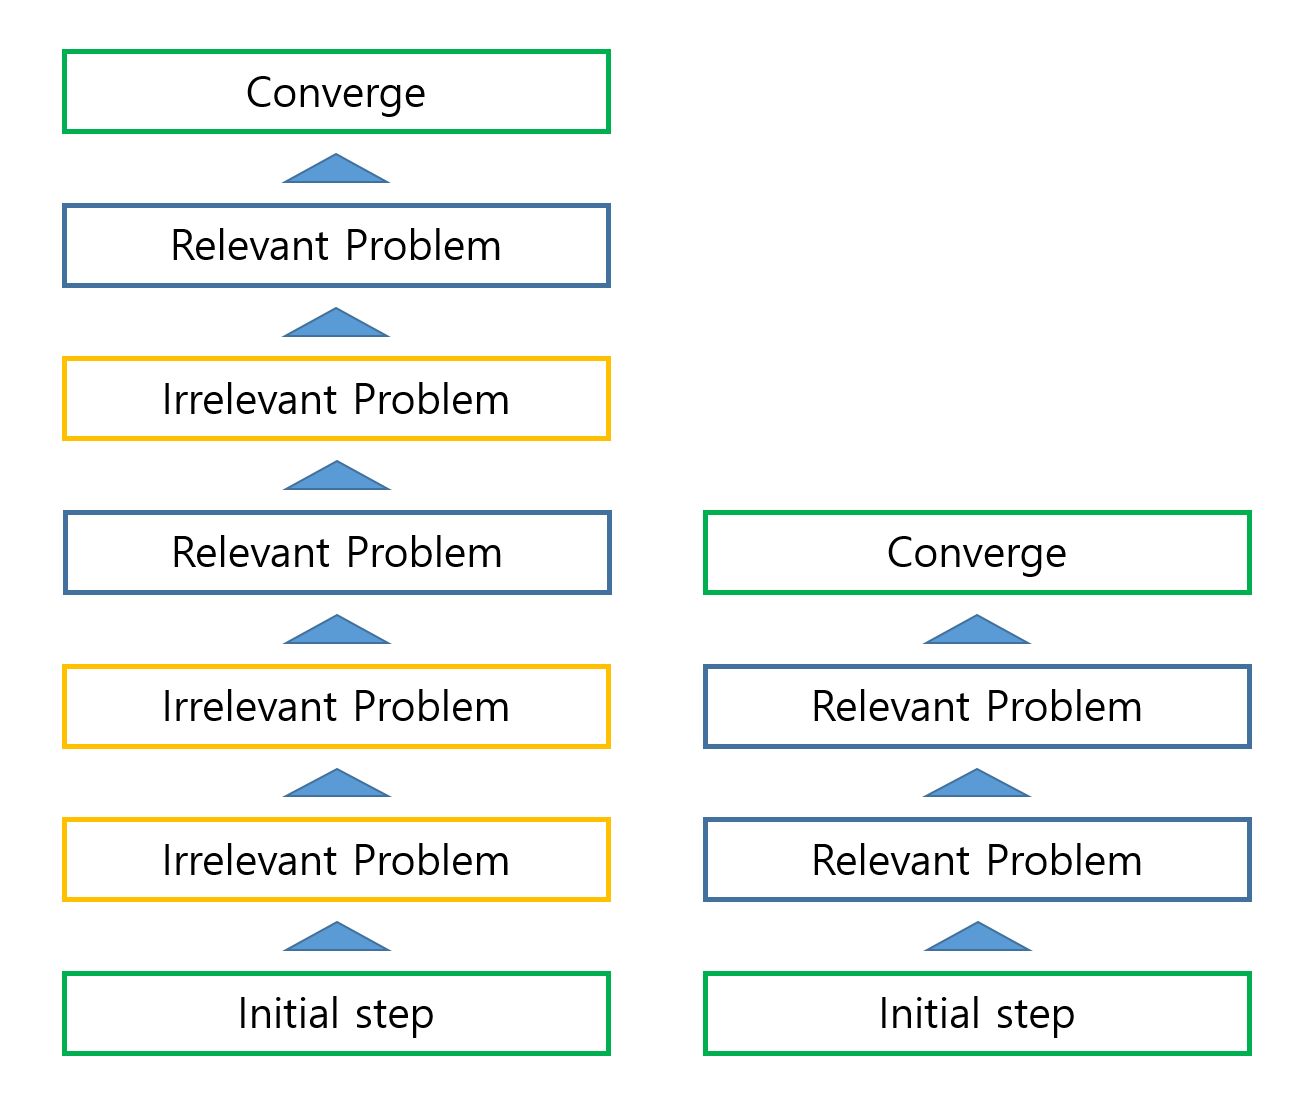
\includegraphics[width=1.0\linewidth]{../figures/non_orderd_vs_ordered_learning}
		\caption{On the left side we show the non-ordered training. It might happen that due to the random selection the model is trained on some irrelevant parts of the problem. If we make sure we only feed training examples to the model that cover relevant parts of the problem we can reach converge faster.}
		\label{fig:nonorderdvsorderedlearning}
	\end{subfigure}%
	~
	\begin{subfigure}{0.5\textwidth}
		\centering
		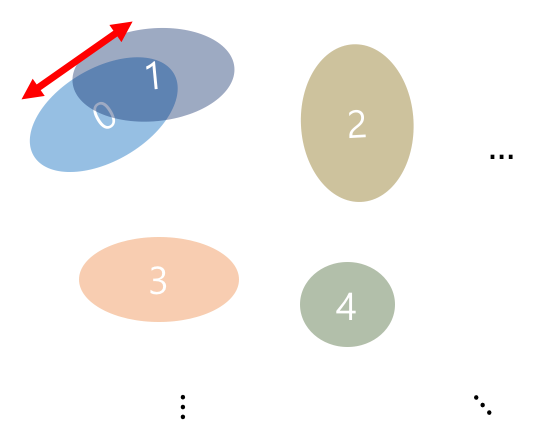
\includegraphics[width=1.0\linewidth]{../figures/optimizing_overlapping_classes}
		\caption{If the model is trained on a batch with the data from class 2, 3 and 4 as seen in the figure, the training loss will be small because those classes are already well clustered and separated. In this situation, the model should focus on the class 1 and 2 to solve the problem.}
		\label{fig:optimizingoverlappingclasses}
	\end{subfigure}
	\caption{How ordering shifts the focus towards the salient classes to train.}
\end{figure}

\subsection{Problem definition}
Briefly, in the beginning of every episode a subset of all possible classes is uniformly/randomly sampled. For this particular episode the subset is now in the main focus during training.

As normally the sampling is done uniformly, it is not always guaranteed that the sampled classes in the subset give sufficient information to improve the model further. 

To overcome this problem we want to modify the uniform sampling by assigning an unique probability to each possible class. The main contribution of our work will be to define a sufficient heuristic or to find a stochastic approach to ensure the networks focus on the not so well explainable parts by assigning a higher selection probability to these classes.
In figure \ref{fig:nonorderdvsorderedlearning} one can see the impact of using an problem specific sampling instead of doing random sampling. While in figure \ref{fig:optimizingoverlappingclasses} an illustration is given on which classes the model should focus in training.

\subsection{Approach}
Right now, we plan to construct a square matrix of all classes. The matrix should correctly represent the overlap between classes. Therefore one possibility would be that each entry of the matrix will be the Jensen-Shannon-Divergence between these two classes in the embedded space. We then continue to calculate a probability either for each class or for each inter-class relationship.

By sampling the classes/relationships with a higher probability we ensure that the loss in the upcoming episode reflects the high overlap for these classes and the network improves on these class sets. To further ensure that non-focused classes do not get worse we may introduce the concept of context classes.

As this a fairly popular sampling problem, we could not choose this simple probabilistic sampling but use a more sophisticated method such as tournament selection.

We could also choose to use KL-divergence instead of Jensen-Shannon-Divergence, so we can save computational power.

Regarding what to sample, from our current point-of-view either class or relationship sampling is possible and investigating which one works better could be one of our possible research questions we want to investigate. In the following we will briefly explain the difference between them.

\subsubsection{Sampling classes}
To ensure a proper distribution, we will sum up the entries of each row/column. As the ultimate goal is to separate the class sets as much as possible we need to take the inverse of the sum because a higher divergence indicates a better separation. Finally, to get a proper distribution we need to normalize the values.

\subsubsection{Sampling relationships}
A different approach for sampling would be not to sample the classes but rather directly the entries in the matrix. This moves the sampling problem from classes to relationship between classes. In this case our sampling process needs to be able to handle already sampled classes through a previous sampled relationship as well as re-weighting the relationship in the matrix whenever a new class was sampled. 

\subsection{Expected results}
We hope we can reduce the training time of the neural network as we draw more attention towards the classes with low separation/high overlap. During the training process the network will focus on these classes and moves them apart (in the embedded space).

\section{Possible Research Direction 2: Clustering New Classes}
Assume we have trained our embedding model only on $S$ classes of the training set from a total of $N$ classes in the data set. If we now feed the rest 
\begin{equation*}
	U = N - S
\end{equation*} 
classes to the model, the model should have learned a mapping in the embedded space based on $S$ classes which places the $U$ unseen classes in a way that they do not collide with each other. This problem is similar to few-shot learning (\cite{edwards2016towards}, \cite{snell2017prototypical}) and incremental learning (\cite{lee2018simple}, \cite{yang2018robust}). 

\subsection{Objectives}
Our goal here is that we now do not know how many $U$ unseen classes are there and try to 
\begin{enumerate}
	\item Classify unseen examples correctly as out-of-distribution
	\item Estimate amount of classes (this prediction should be N-K)
	\item Predict which samples belong to which class (we correctly reproduce the labels based on the true clustering) -- e.g. this could be realized with the expectation maximization algorithm, given the previous tasks were performed correctly
\end{enumerate}

In figure \ref{fig:detectionofunseenclasses} one can see the optimal behavior for our model in the embedded space.

\begin{figure}
	\centering
	\begin{subfigure}[h]{0.5\textwidth}
		\centering
		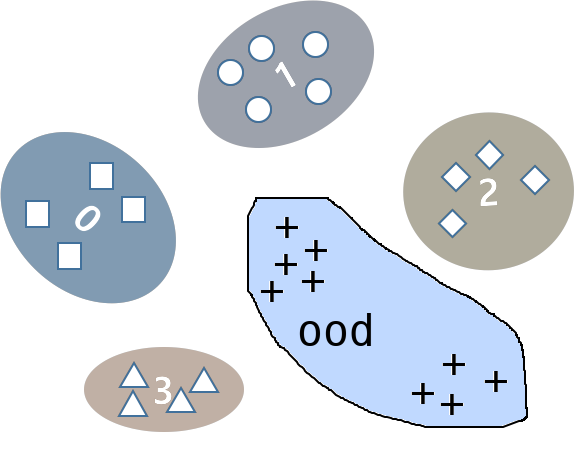
\includegraphics[width=0.9\linewidth]{../figures/detection_of_unseen_classes_unclassified}
		\caption{We correctly classify the new examples as out-of-distribution (ood). Here indicated with plus.}
		\label{fig:detectionofunseenclassesunclassified}
	\end{subfigure}%
	~ 
	\begin{subfigure}[h]{0.5\textwidth}
		\centering
		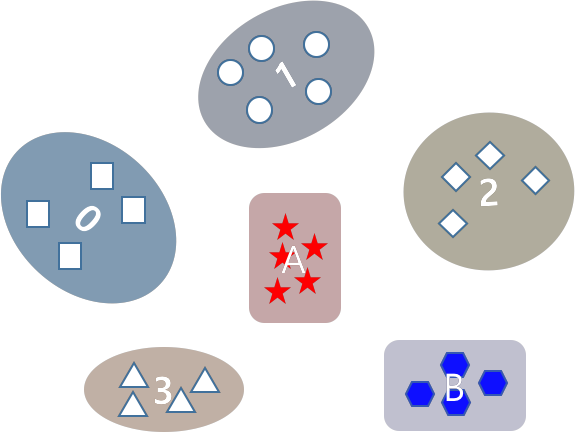
\includegraphics[width=0.9\linewidth]{../figures/detection_of_unseen_classes_classified}
		\caption{We can correctly cluster the out-of-distribution examples as an unseen training example.}
		\label{fig:detectionofunseenclassesclassified}
	\end{subfigure}
	\caption{In this figure one can see the embedded space for a problem with $S=4$ and $U=2$. In this case the seen classes are 0, 1, 2, 3, while examples from the classes A and B were not presented to the model during training.}
	\label{fig:detectionofunseenclasses}
\end{figure}

\subsection{Expected results}
We hope we are able to correctly detect and cluster new examples which are drawn from the same data set. In \cite{yang2018robust} the authors trained their model on the MNIST data set and feed images from the CIFAR data set to see if their model correctly puts them in a separate area in the embedding space. Unfortunately their model is not able to place each CIFAR-class at a different location but rather all in the same spot. This makes a clustering impossible. When comparing to this we expect that training on 80 classes and testing on 20 classes of the CIFAR100-set will place the remaining classes in a more meaningful.

\section{Baseline Implementation}

As our baseline implementation we plan to build a very small network consisting of the following parts: Use a feature extractor (like ResNet, VGGNet) combined with a embedding space encoder. 

Using this encoded vector, we could then measure the probability for sampling training examples based on the correlation between classes. Therefore, the model is able to use the training data in a reasonable order by choosing the training examples based on the probability for either the class or the relationship. 

For our second research direction of finding out-of-distribution examples we can use the embedded vector to compare it to the given distributions of the known classes. We could introduce a simple threshold which tells us whether the example was out-of-distribution or belongs to a class. This is similar to the approach in \cite{yang2018robust}.

We might also borrow the structure of the network and the loss calculation from \cite{edwards2016towards} or \cite{snell2017prototypical}.


\bibliography{../literature.bib}
\bibliographystyle{../icml2018_style/icml2018}

\end{document}
